%  This LaTeX template is based on T.J. Hitchman's work which is itself based on Dana Ernst's template.  
% 
% --------------------------------------------------------------
% Skip this stuff, and head down to where it says "Start here"
% --------------------------------------------------------------

\documentclass[12pt]{article}
\usepackage[margin=1in]{geometry} 
\usepackage{amsmath,amsthm,amssymb}
\usepackage{graphicx}
\usepackage{listings}
\usepackage{hyperref}
\usepackage[nottoc]{tocbibind}
\usepackage{xurl}
\PassOptionsToPackage{hyphens}{url}\usepackage{hyperref}
\hypersetup{
	colorlinks=true,
	linkcolor=blue,
	filecolor=magenta,      
	urlcolor=cyan,
}
\newenvironment{statement}[2][Statement]{\begin{trivlist}
		\item[\hskip \labelsep {\bfseries #1}\hskip \labelsep {\bfseries #2.}]}{\end{trivlist}}
\begin{document} 
\title{Final Report}
\author{Eric L. Lee, Shu-Hao Chang, Yu-Cheng Weng, Can Jiang} 
\maketitle

\section{Abstract}

In this report, we focus on solving link prediction problem. The core problem of link prediction is to extract or learn features for each link or we cannot use machine learning model to solve the problem. We survey several methods and categorize these methods into three categories in our proposal which is heuristic method, latent feature method and subgraph sampling method.
Due to the time limit, we haven't implemented subgraph sampling method when we submitted the report. However, we've implemented heuristic method and latent feature method. Besides, we do a very careful experiments on 8 different data sets and find some very interesting facts seldom mentioned in the paper.  We also find a mistake about the result of matrix factorization in a series of paper published in KDD 2017 and NIPS 2018. We have notified the author and prevent mistakes in the future publication. Through the conversation with the authors, we think it is actually a mistake that very easy to commit if we don't pay attention to the implementation of machine learning package. In fact, the two paper have a total 80 citations and no one find this mistake. We will also illustrate this mistake in the Matrix Factorization section.
\\ \\
Our report will arrange in the following way. Chapter 2 is the introduction of our problem and Chapter 3 is a section of how to reproduce our result. Chapter 4 is some data analysis we've done do our data set. In Chapter 5, we wlll talk about some simple heuristic and our evaluation method. 

\section{Introduction to Link Prediction Problem}
Link prediction is a task to predict whether there will be an edge between two nodes. Link prediction is actually very different from an usaual machine learning task by the following three characteristics:
\\ \\
1. We don't have any feature vector predefined in our graph. 
\\ \\
2. Link prediction is a ranking problem.
\\ \\
3. The positive data is much more than the negative data. 
\\  \\
The first characteristics is seldom encounted when we face other machine learning problem which makes link prediction very unique.  \\
To make link prediction a machine learning problem. There are three ways to generate(or learn) feature vector. \\
1. Heuristic \\ 
This is the most simple way, but it is actually a very effective way. And there are some very famous heuristic such as common neighbors, Katz similarity, Preferentail Attachment, ... etc.  We will discuss this method from chapter 5 to chapter 7. \\ \\
2. Latent Feature Method \\
This method is to use factorization model(a.k.a Matrix Factorization) \cite{mf}. We give each node a latent feature vector and use the inner product be the probability whether the node will have the link. This method has a great performance in recommendation problem (link prediction in biparitite graph). We want to test wheter it will have the same great performance when it comes to a much more general link prediction problem. 
\\
We will discuss this method in Chapter 8.
\\ \\
3. Subgraph Sampling Method \\ 
Subgraph Sampling approach is to sample a set of subgraph and enumerate all the nodes in each subgraph. As a result, the adjacency matrix in each subgraph of these subgraph can be the feature vector for machine learning approach. In fact, there are two recent works proposed in KDD 2017 \cite{lp2017} and NIPS 2018 \cite{lp2018} using this method. 
\\ 
To illustrate the idea of subgraph sampling, let us draw an example in Figure \ref{fig:subsample}. 
\\
The second and third characteristic actually will let link prediction need to have an unique way to evaluate model and we will discuss this in Chapter 5.2. 
\\
\begin{figure}[h]
	\centering
	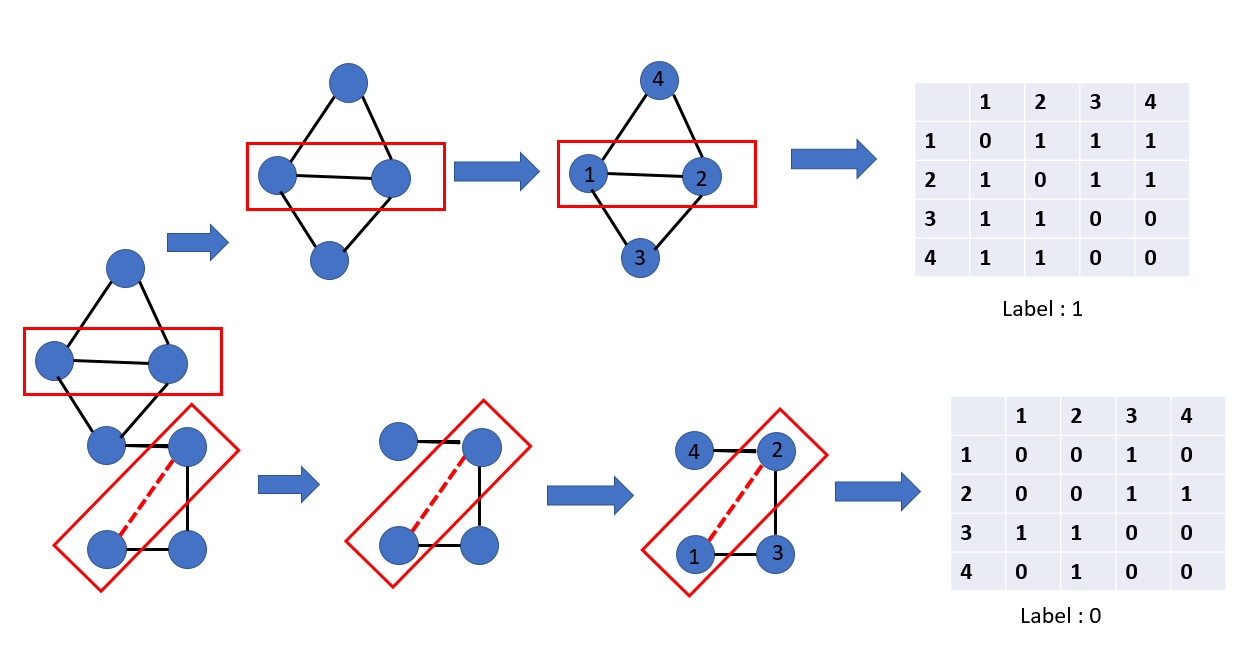
\includegraphics[scale=0.3]{subgraph_sampling_approach}
	\caption{subgraph sampling method}
	\label{fig:subsample}
\end{figure}

\section{How to Reproduce Our Result}
We believe that reproducibility is very important when it comes to research. Thus, we carefully recorded all of our experiment results on Github. All the results presented in the following sections can be easily reproduced using this github repository: 
\\
\\
\url{https://github.com/miamiasheep/Purdue\_ML\_Course\_Project}
\\
\\
And all of our experiements can be reproduced by following the instruction of README. If you have any problems of reproducing the experiments, please feel free to contact me by posting an issue or sending me an email at lee3388@purude.edu.

\section{Data Analysis}

\subsection {Data Set}
We collect 8 different datasets which are all unique and have different characteristics. Table \ref{tab:info} shows basic statistics of each data set.
\subsubsection{Facebook}
This is a dataset downloaded from SNAP(Staford NEtwork Analysis Project)\cite{snapnets}. The data is an egonet in facebook. Each node represents an account in Facebook and each link represents friendship in Facebook.
\subsubsection{Power}
Power is  an electrical grid of western US\cite{small_world}.
\subsubsection{NS}
NS is a collaboration network of resarchers who publish paper on network sciences \cite{Newman_2006}.
\subsubsection{PB}
PB is a network of US political blogs.\cite{pb}
\subsubsection{Router}
Router is a router-level Internet.\cite{router}
\subsubsection{USAir}
USAir is a network of US air lines. \cite{usair}
\subsubsection{Yeast}
Yeast is a protein-protein interaction network in yeast.\cite{yeast}

\subsubsection{Celegan}
Celegan is a neural network of C. elegans.\cite{small_world}

\begin{table}
	\begin{center}
		\begin{tabular}{|c|c|c|c|c|}
			\hline
			data set & nodes & edges & average degree & max degree \\
			Facebook & 4039 & 88234 & 21.85 & 1045 \\
			Power & 4941 & 6595 & 1.33 & 19 \\
			NS & 1461 & 2742 & 1.87 & 34 \\
			PB & 1222 & 16714 & 13.68 & 351 \\
			Router & 5022 & 6258 & 1.26 & 106 \\
			USAir & 332 & 2126 & 6.40 & 139 \\
			Yeast & 2375 & 11683 & 4.91 & 118 \\
			Arxiv & 18772 & 198110 & 10.55 & 504 \\
			Celegan & 297 & 2148 & 7.23 & 134 \\
			\hline 
		\end{tabular}
		\caption{Basic Information of different data set}
		\label{tab:info}
	\end{center}
\end{table}

\subsection{Visualizing Our Data Set}
We implemented a tool to visualize our datasets. And all of our visualization graphs can be seen in the following link:
\\
\\
\url{https://github.com/miamiasheep/Purdue_ML_Course_Project/tree/master/graph}
\\
\\
Since the network is too big and it is hard to find any clue regarding the network structure if we draw all the edges and nodes, we only sampled a small portion of the network on every dataset.
\\
\\
By visualizing our data sets, we can see that the characteristic of each data is actually very different. Let's take Facebook (figure\ref{fig:facebook}) and Router (figure\ref{fig:Router}) as examples. Facebook dataset has multiple triangles in the middle of the network. In contrast, Router has no triangle in the data set.


\begin{figure}[h]
	\centering
	\includegraphics[scale=0.3]{Facebook}
	\caption{facebook}
	\label{fig:facebook}
\end{figure}

\begin{figure}[h]
	\centering
	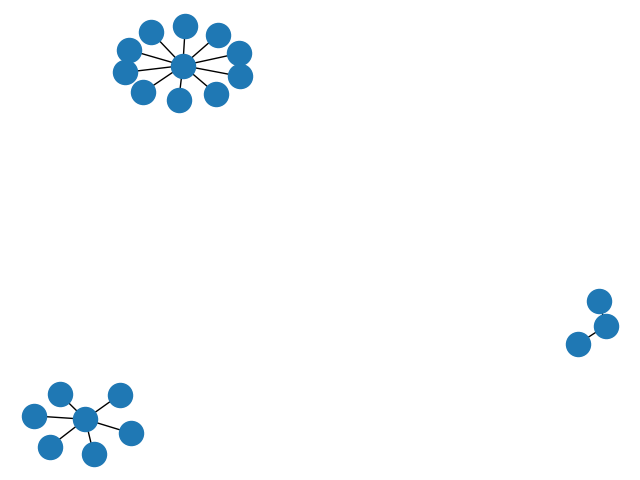
\includegraphics[scale=0.3]{Router}
	\caption{Router}
	\label{fig:Router}
\end{figure}
\section{Evaluation and Result}

\subsection{Baselines}
For the following sections, we denote x and y as two nodes, between which we want to predict if there is a link. And we denote the set of neighbors of x as N(x). We implemented six very common heuristics. And in table \ref{tab:method}, we organized the formulas of the six heuristics. \\
\subsubsection{Common Neighbors(CN)}
It is a very simple heuristic. The intuition is that the more common neighbors the two nodes have, the more likely that there is a link between them. The score can be calculated as $|N(x) \cap N(y)|$.
\subsubsection{Jaccard(JC)}
It is very similar to common neighbors except that Jaccard considers the fact that two higher degree nodes unsurprisingly tend to have more common nodes. Thus, if two lower degree nodes have common neighbors, maybe they really have a strong relationship. The score can be calculated as $\frac{|N(x) \cap N(y)|}{|N(x) \cup N(y)|}$
\subsubsection{Adamic Adar(AA)}
It is also very similar to common neighbors. It assumes that a low degree common neighbor have more contribution to the probability of a link between x and y. Thus, the score divides the weight of each common neighbor by the logarithm of its degree. It is actually very similar to TFIDF. And we can calculate the Adamic Adar by $\sum_{z \in N(x) \cap N(y)}{\frac{1}{log(|N(z)|)}}$
\subsubsection{Total Neighbors(TN)}
It is the simplest baseline, which is just summing up the total size of neighbors of x and y. It can be calculated as $|N(x)| + |N(y)|$
\subsubsection{Preferential Attachment(PA)}
It is assumed that a high degree node have more chances to have a link with other nodes. Preferential Attachment calculate the product of degree of x and y. It can be calculated as $|N(x)| * |N(y)|$
\subsubsection{Page Rank(PG)}
It is very similar to PA. But instead of using the product of nodes' degrees, it uses the product of two nodes' scores derived from performing page rank on our network. Since the product can be very small, we use the sum of logarithm instead. Let $r_x$ be the score of x after performing page rank and $r_y$ be the score of y after page rank. It can be calculated as $\log{r_x} + \log{r_y}$
\begin{table}
	\begin{center}
		\begin{tabular}{|c|c|}
			\hline
			method & description \\
			\hline
			common neighbor(CN) & $|N(x) \cap N(y)|$ \\
			Jaccard(JC) & $\frac{|N(x) \cap N(y)|}{|N(x) \cup N(y)|}$ \\
			Adamic and Adar(AA) & $\sum_{z \in N(x) \cap N(y)}{\frac{1}{log(|N(z)|)}}$ \\
			Total Neighbor(TN) & $|N(x)| + |N(y)|$ \\
			Preferentail Attachment (PA) & $|N(x)| * |N(y)|$ \\
			Page Rank(PR)  & $\log{r_x} + \log{r_y}$ \\	
			\hline
		\end{tabular}
	\end{center}
	\caption{link prediction methods}
	\label{tab:method}
\end{table}

\subsection{Evaluation}
Evaluation is not trivial when it comes to link prediction problems. If we want to evaluate all pairs of nodes, it will need O($N^2$) predictions, where N is the size of the nodes. And even for a small graph with 1000 nodes in testing set, the evaluation time can be really long because we have to make 1000 * 999 /2 predictions. In fact, finding a fair and effective evaluation is also a research topic. Ryan and Nitech published a paper \cite{eval} about how to evaluate a link prediction problem. We choose the most common way to evaluate our model: Down-sampling negative samples. (By negative samples, we mean a pair of nodes with no link between them. In link prediction problems, negative samples are usually way more than positive ones.)
\\
\\
First, we randomly divided our edges into training, validation and testing. The ratio is 0.8:0.1:0.1. Training set is for training while validation set is only for grid search for the best parameters. And testing set is for evaluation of our model. 
\\
\\
Second, we randomly sampled negative samples for validation and testing set. The sample size is equal to the set size.
\\
\\
Third, we train the models using training set, and tuned our model using validation set, and evaluate the models to our testing set. The higher score a pair gets, the higher the ranking it is and the more possible that there would be a link between them. For evaluation, we used the ranking metrics. We mainly used AUC-ROC score (area under Receiver Operating Characteristics curve, abbreviated to AUC here). AUC has a very good characteristic that the sampling AUC is actually an approximation of actual AUC even if we do down-sampling. 
\\
\\
We also implemented f1@k score as an evaluation metric. For the parameter k, we tentatively set the k equal to the size of positive samples. For this k, recall is actually equal to precision. And f1@k thus has a very intuitive physical meaning: the accuracy of finding all of the missing links given the size of missing links. In the future, we'll try to set different k's and see the influence of them. 
\\
\\
Also, something to note here is that some nodes may only exist in validation or testing set but not in training set. We discarded the pairs of nodes where at least one node is not in the training set when evaluating, i.e., We only considered pairs of which both nodes are in the training set.


\section{Result and Discussion of Heuristic Methods}
\begin{table}
	\begin{center}
		\begin{tabular}{|c|c|c|c|c|c|c|}
			\hline
			Data Set & CN & JAC & AA & PA  & TN & PG \\
			\hline
			Celegans&0.8314&0.7669&0.8443&0.7554&0.734&0.7587\\
			facebook&0.9882&0.9863&0.9893&0.8324&0.7345&0.8085\\
			NS&0.9742&0.9747&0.9741&0.6803&0.5204&0.5206\\
			PB&0.9152&0.8669&0.9176&0.908&0.8776&0.9094\\
			Power&0.5965&0.5964&0.5965&0.528&0.5198&0.5536\\
			Router&0.6109&0.6102&0.6111&0.9298&0.9198&0.9418\\
			USAir&0.9509&0.9164&0.9626&0.9021&0.868&0.8971\\
			Yeast&0.902&0.901&0.9029&0.8561&0.7926&0.8488\\
			\hline
		\end{tabular}
	\end{center}
	\caption{AUC of the six baselines}
	\label{tab:auc}
\end{table}

\begin{table}
	\begin{center}
		\begin{tabular}{|c|c|c|c|c|c|c|}
			\hline
			Data Set & CN & JAC & AA & PA & TN & PG \\
			\hline
			Celegans&0.7407&0.5926&0.713&0.5694&0.5787&0.5833\\
			facebook&0.9546&0.9312&0.9544&0.6742&0.5618&0.6455\\
			NS&0.9524&0.9524&0.9524&0.5281&0.3939&0.3723\\
			PB&0.8052&0.6927&0.801&0.7762&0.7223&0.7792\\
			Power&0.1947&0.1947&0.1947&0.396&0.3518&0.3252\\
			Router&0.2279&0.2279&0.2279&0.761&0.7574&0.7721\\
			USAir&0.8278&0.7608&0.8612&0.799&0.7799&0.7608\\
			Yeast&0.815&0.815&0.815&0.7024&0.6184&0.6944\\
			\hline
		\end{tabular}
	\end{center}
	\caption{F1 score of the six baselines}
	\label{tab:f1}
\end{table}

Table \ref{tab:auc} shows AUC's of the six different baselines and Table \ref{tab:f1} shows the F1 scores.
\\
\\
According to the result above, we can see that no heuristic method can outperform all other heuristics, and that Adamic Adar(AA), Jaccard, and common neighbors perform pretty well in the Facebook and NS dataset. However, for Power and Router dataset, the results of common neighbor based methods are pretty bad. This is not surprising because in Power and Router dataset, there are so few triangles that the methods aren't able to achieve good performances. 
\\
\\
To achieve a better result, we want to resort to machine learning approach. Instead of designing a heuristic before actually seeing the data, we want to train our model using the existing link in the training data. The main problem of machine learning approach is to find the feature vector for each node. 

\section{Matrix Factorization}

In this section, we try to apply Matrix Factorization to link prediction. Matrix Factorization works by decomposing user-item interaction matrix into the product of two lower dimensionality of rectangular matrices. It is very popular in recommendation system problem. Let the user-item interaction be the matrix R. And the first matrix be P and the second matrix be Q.  
\\
\begin{equation}
\min_{P,Q}{\sum_{(u,i)}{L(R_{u,i}, P_uQ_i^T)}}
\end{equation}
where L is the loss function we can define. \\
\\
For example, the following equation is a example of using square error. \\
\begin{equation}
\min_{P,Q}{\sum_{(u,i)}{(R_{u,i}-P_uQ_i^T)^2}}
\end{equation}
However, the link prediction goal is the ranking not square error. So, we adopt Bayesian Personal Ranking\cite{bpr} in this problem. Denote P is the user matrix, Q is the item matrix. And (u,i) is the 
\begin{equation}
\min_{P,Q} \sum_{(u,i,j)\in D_s}\log(1+e^{-P_u(Q_i^T - Q_j^T)})
\end{equation}

All of the implementation can be found in libmf\cite{libmf} and we directly use libmf in our experiment.

\subsection{A Miastake Using Matrix Factorization}
We find that we should be very carefully when apply matrix factorization to solve link prediction problem.
When we do survey related paper, we find that some paper use the matrix factorization in the wrong way. And the mistake is still existing in a very recent NIPS paper. The paper was accepted in KDD 2017 and then submitted in NIPS 2018 uses this incorrect result and being accepted without notice the bug. We then contact the author and  find that we are the first one to find this bug. Because the paper is already cited by 50 papers, we think it might be a bug that not so easy to find. So, we want to point out this mistake in the following section and our final project presentation.   

\subsection{Zero Predictions Problem}
Matrix Factorization is very popular in solving recommendation problem which can be one of link prediction problem. The only difference is that recommendation problem focus on the bipartite graph. 
\\
Obviously, matrix factorzation can also solve link prediction problem that is not bipartite. The most intuitive way to do this is: 
\\
1. Read all the edges to form the tuple in set O.
\\
2. Apply MF library and get the MF model.
\\
3. Generate predictions using this MF model.
\\
\\
However, it is not the correct way to use matrix factorization. In fact, it will yield a very bad result especially for the graph has low average degree. 
\\
However, Matrix Factorization performs bad not because it is not suitable for this problem. Matrix Factorization performs bad because it predicts many zeros. Apparently, there are something going wrong here. Table \ref{tab:zero} shows the percentage of zero prdictions of each data set. 
\\
\begin{table}
	\begin{center}
		\begin{tabular}{|c|c|c|c|}
			\hline
			Data Set & zeros & testing size & percentage(\%) \\
			\hline
			Celegans&42&431&9.74 \\
			facebook&1008&17556&5.74 \\
			NS&113&477&23.69 \\
			PB&685&3237&21.16 \\
			Power&338&1027&32.91 \\
			Router&282&724&38.95 \\
			USAir&96&414&23.19 \\
			Yeast&404&2192&18.43 \\
			\hline
		\end{tabular}
	\end{center}
	\caption{zero predictions in each data set}
	\label{tab:zero}
\end{table}

\subsection {Update Rules of Matrix Factorization}


\subsection{Two ways to solve this problem}

\subsubsection{Duplicate data}
The most simple way to solve the problem is to duplicate the training data. For each edge (x,y), we create a new edge (y,x) in the training set. It will solve the problem. Table \ref{tab:dup} shows the improvement of doing this modification. We can see that it helps a lot for low degree graph. For Power data set, there is about 30\% improvement. 

\begin{table}
	\begin{center}
		\begin{tabular}{|c|c|c|c|}
			\hline
			Data Set & mfWrong & mfDup & Improvement(\%) \\
			\hline
			Celegans&0.7502&0.7978&6.34\\
			facebook&0.9797&0.9799&0.02\\
			NS&0.8081&0.9364&15.88\\
			PB&0.8675&0.8361&-3.62\\
			Power&0.5307&0.6985&31.62\\
			Router&0.7321&0.8271&12.98\\
			USAir&0.8183&0.8193&0.12\\
			Yeast&0.924&0.9557&3.43\\
			\hline
		\end{tabular}
	\end{center}
	\caption{zero predictions in each data set}
	\label{tab:dup}
\end{table}



\bibliographystyle{acm}
\bibliography{final_report}
	
	
\end{document}